This chapter of the bachelor's thesis serves to introduce the fundamental concepts for the inception of smart homes, such as the Internet of Things, home automation and also edge computing. Moreover, it delves into the origins and main principles of the Zero Trust security model, while later describing the essential concepts and technologies necessary for understanding the thesis work.

\section{Smart Homes}
In today's digital world, the practice of devices and sensors being connected over the Internet to integrate real-time monitoring and a degree of smart assistance with appliances in a given environment is becoming more prevalent, especially into private residences. This trend marks the rise of the smart home, also known as a smart home system (SHS), with the goal to automate certain mundane tasks and improve the quality of life in a household. By the end of the 2020s, the number of smart homes is projected to reach 1.9 billion people \cite{smarthome_report}, indicating a growing market for the integration of smart appliances at home.\\
With regard to these numbers, the attack surface of home networks is consequently bound to expand as well, making them a prime target for malicious actors, usually hackers to collect user data and thus compromise user privacy. Before diving deeper into the topic of smart home security, this section provides a brief overview on the topics of IoT and Home Automation as foundational concepts for smart homes, to allow the reader to understand the bigger picture.

\subsection{Internet of Things (IoT)}
At first, the term “Internet of Things” (IoT) referred to the effort to combine radio-frequency identification (RFID) and different types of sensors to provide additional functionality to generic objects \cite{ng_internet--things_2017}. However, over the years the concept of IoT has proceeded to expand on the idea of connectivity and evolved into a network of interoperable devices, which function as an amalgamation of household, transport, and monitoring devices with sensors, which contributes to the tremendous exchange known as big data, thus defining the modern foundations for the IoT \cite{khedekar_home_2017}. A typical example for an IoT device in the context of smart homes is a mobile TVOC \cite{understanding_tvoc} air quality sensor, which gathers the raw data about the temperature, humidity and TVOC levels in the air and transmits it to a designated network gateway connected to the home network \cite{aqara_monitor}.

\subsection{Home Automation}
Home Automation (HA) is broadly defined as the use of sensors and other smart devices together with predetermined behaviour with the objective to enable a domestic environment to autonomically and remotely accomplish different sets of operations \cite{smart_home_automation_iot_edge}. This notion, in conjunction with IoT technology and HA-enabling software, e.g. Home Assistant \cite{home_assistant}, is what constitutes the basic structure of a smart home system. Figure 2.1 depicts a high-level diagram of a smart home with different IoT-based home automations. It should also be noted that while each node can be treated as a separate operation, HA is most successfully realized with a set of various automations. 

\begin{figure}[H]
	\centering
	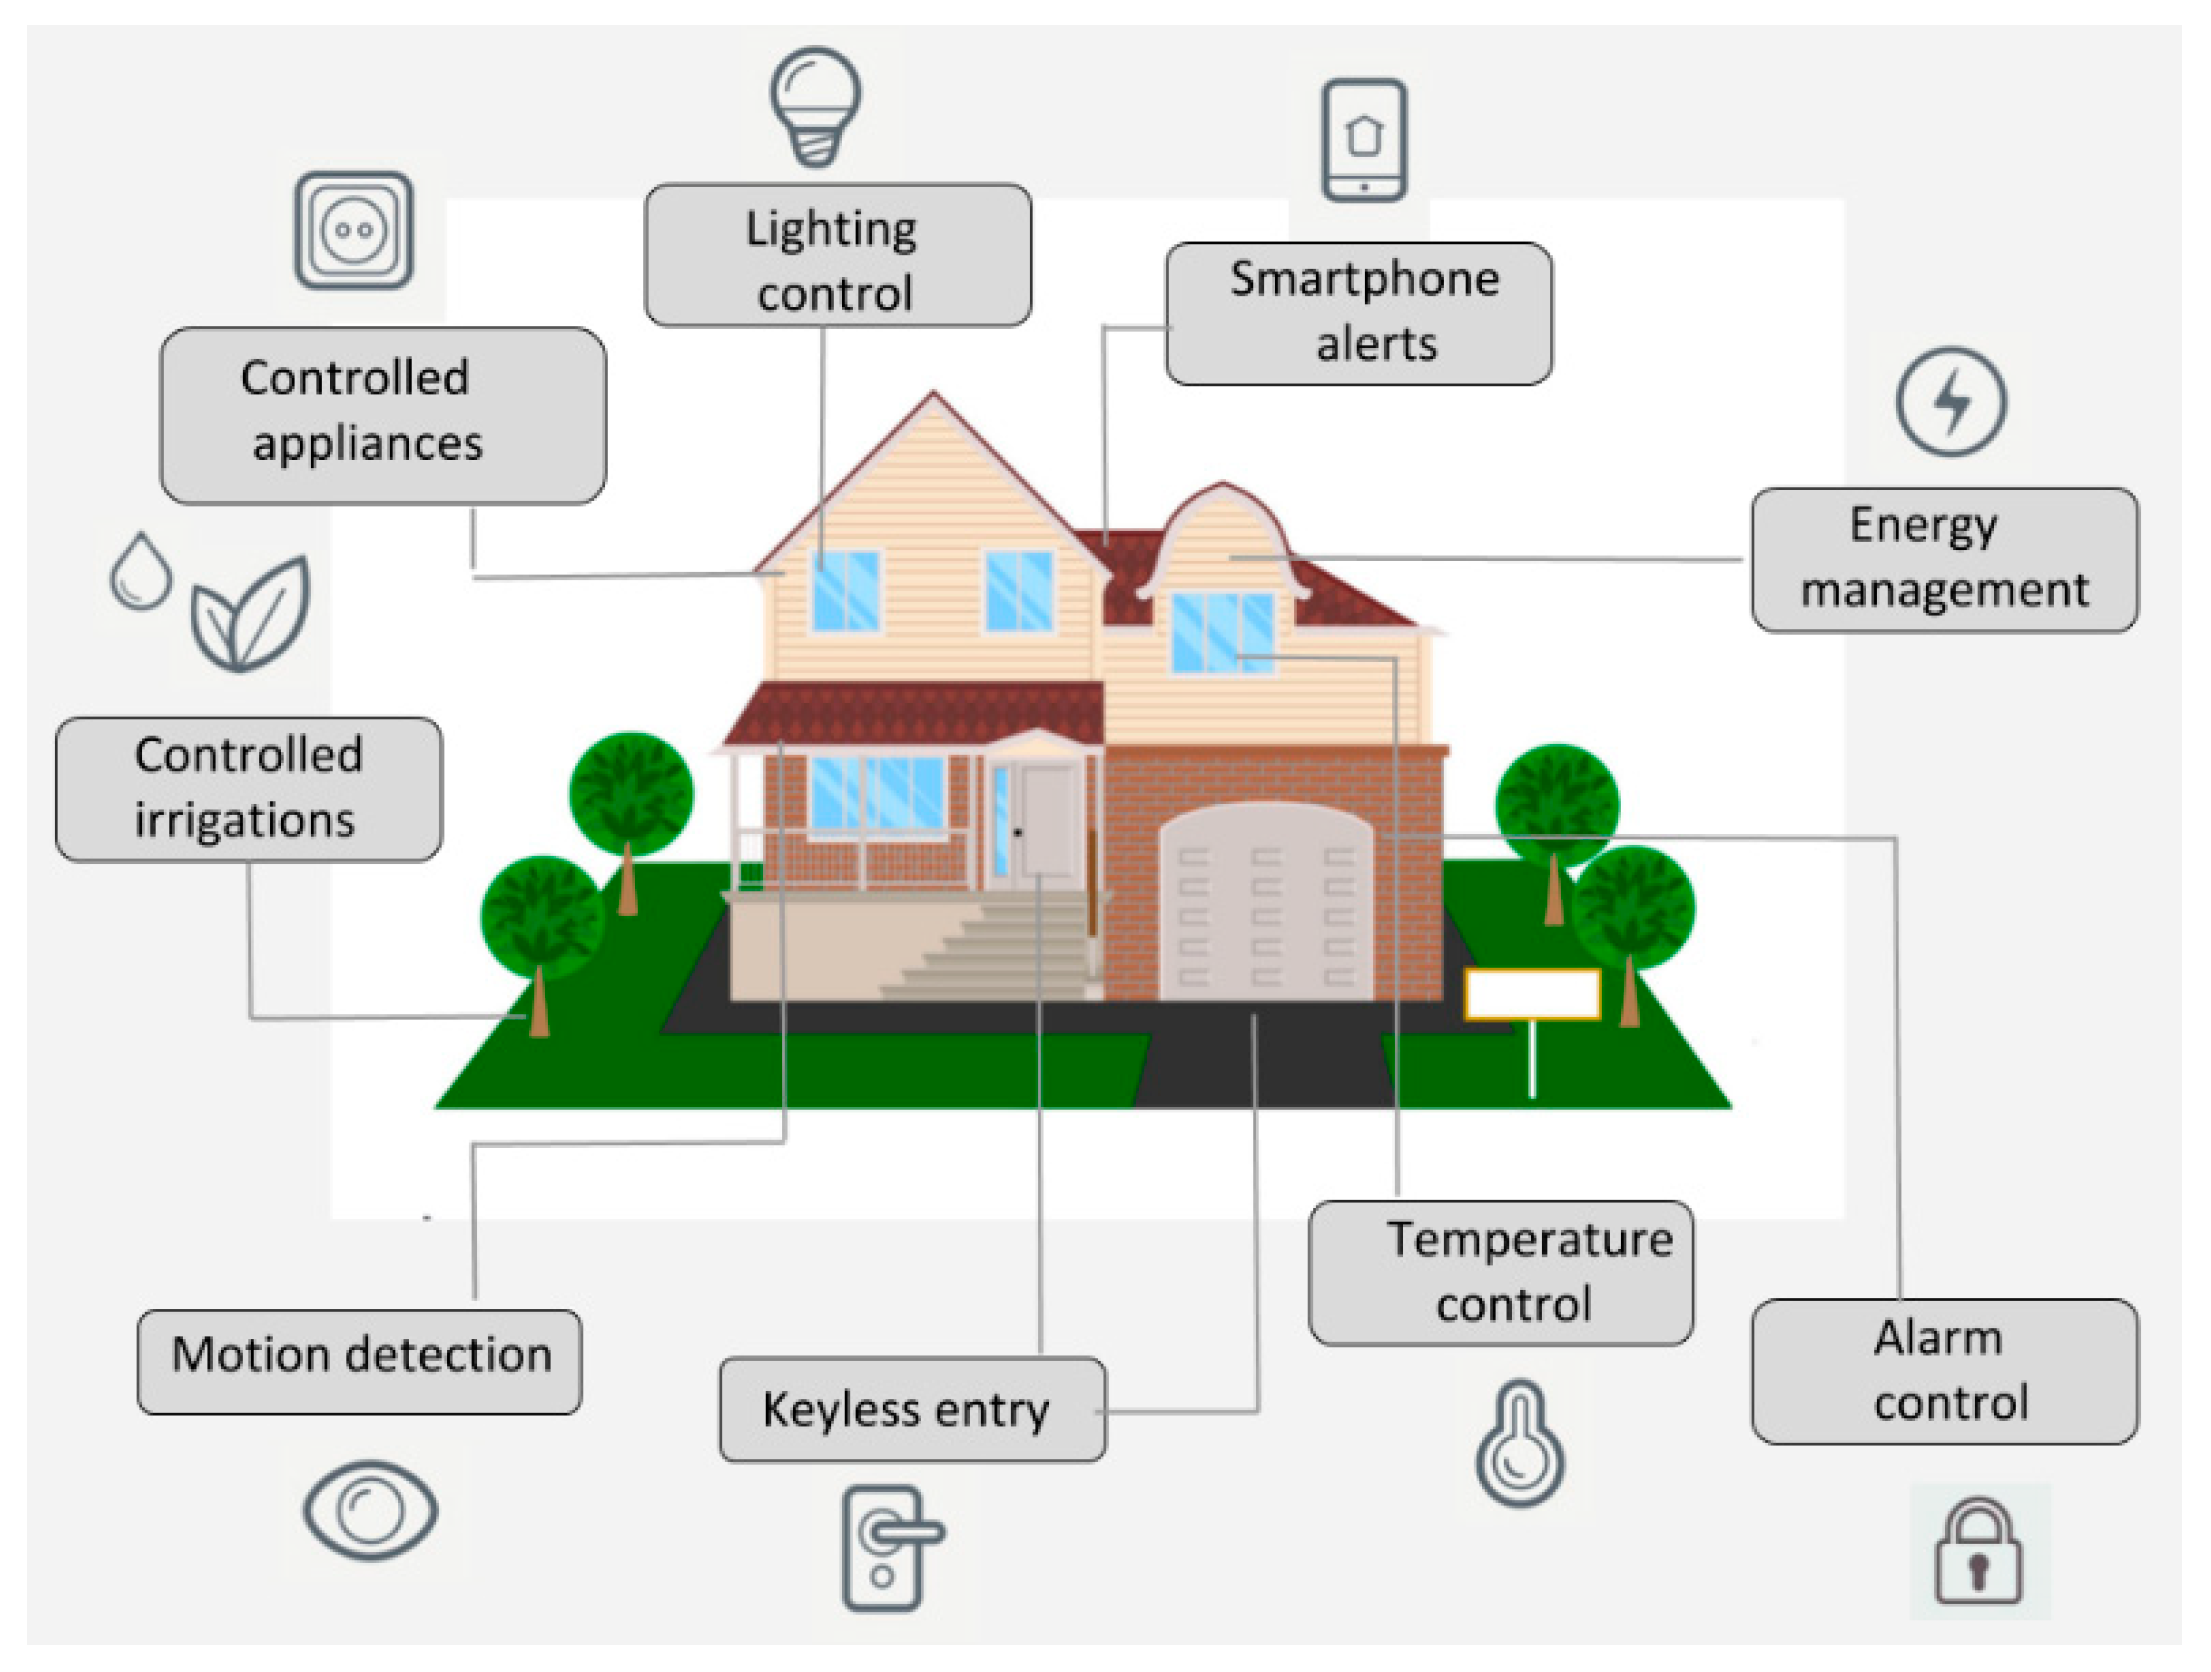
\includegraphics[width=0.7 \linewidth]{Images/sensors-21-03784-g001.png}
	\caption{A smart home with several examples of HA}
	\label{fig:Home_Auto_Applications}
    \cite{stolojescu-crisan_iot-based_2021}
\end{figure}

For instance, temperature control can be implemented via a smart thermostat device, which regulates the internal temperature of the home according to the information gathered from motion sensors. Moreover, a simple energy management automation can monitor all controlled smart lights and appliances in the house, sending a weekly notification from the HA software with the estimated electricity costs. These are two basic examples, and yet the depth of home automation is in actuality merely limited by the amount of smart devices in the home and the creativity of end users. 

\subsection{Edge Computing}
Being often mentioned together with IoT, Edge computing involves the implementation of all computing tasks on the “edge” of the network, which can be defined as any computing and network resource between the source of the data and a cloud data centre \cite{edge_comp}. The premise of this approach is that, as the majority of data is produced on the edge of the network, it would be more efficient for it to be processed there. As stated in \cite{edge_comp}, the results based on a proof-of-concept platform for face recognition are a significant reduction of response times and energy consumption. In this context, the idea to implement edge computing in a smart home security architecture offers interesting insights in regard to security and safety \cite{edge_comp_sec}, however as this thesis primarily focuses on the Zero Trust security model for a smart home network these are only mentioned in the “Outlook” section of the last chapter.

\section{Zero Trust Security Model}
The zero trust security model is defined by the assumption that a network has already been breached and as a result, trust granted to users within the network must continuously be subject to reevaluation. The function of this security paradigm is to limit the implicit trust, which comes with perimeter-based security measures, and thus adjust the network's security to the constant analysis of the risks associated with its users and resources.\\
A typical zero trust architecture (ZTA) would include the provision of resources (e.g. data, services, applications) for subjects in the network on an as-needed basis, as well as the constant authentication of the identity and security of each of those subjects. In stark contrast to that, traditional network architectures, focused on the defence of their perimeters, provide authorized subjects with a broad array of resources once they are in the network, making way for lateral movement within \cite{lateral_movement}.

\subsection{Origins}
The concept of Zero Trust security was first devised to mitigate the limitations coming from perimeter-based security models. The term was first formalized by the analyst John Kindervag in 2010, as he came to the following conclusion -- it is possible for attackers to take advantage of and subsequently infiltrate an organization's network to access the company's sensitive data, all because of the implicit trust placed on the internal network traffic \cite{zt_origins_article}. This, in turn, prompted the paradigm shift from placing trust in both the outside and inside perimeters of a network into making sure that the separate entities, e.g. users, applications, etc., are secure.
Since its inception, the Zero Trust model has become widely recognized, with many organizations aiming to overview and adopt its principles with the intention of strengthening their own security posture. In 2020, the National Institute of Standards and Technology (NIST) published the NIST Special Publication 800-207, which provides a detailed overview of ZT architectures as a whole, including their logical components, possible deployment scenarios and related threats, along with a framework for Zero Trust architecture design \cite{zero-trust-nist-rose-2020}.

\subsection{Core Components}
The Zero Trust model integrates several core components to achieve the task of strengthening network security and reduce the number of unauthorized access occurrences and the size of attack surface. As thoroughly described in \cite{zt_origins_article}, the main components of the ZT model are as follows:

\subsubsection{Multi-Factor Authentication (MFA)}
Considered foundational for the implementation of Zero Trust, Multi-Factor Authentication is the practice of utilizing two or more authentication factors to verify the identity of users and thus grant access to certain resources. As part of this process, authentication factors are divided into one of three groups to identify users, outlined in \cite{gilman_zero_2017}:
\begin{itemize}
    \item Something the user alone knows (e.g., a password or PIN)
    \item A physical credential only the user can provide (e.g., a one-time passcode)
    \item An inherent trait of the user (e.g., a fingerprint or face scan)
\end{itemize}

Figure 2.2 depicts the overall workflow of MFA in its most common configuration with two authentication factors. Should one of the factors not be verified correctly, this means that the identity of the user cannot be properly confirmed, in turn making it invalid.\\
MFA benefits the security of the Zero Trust model by introducing an additional factor, making it harder for attackers to replicate and assume the identity of users. Moreover, should one of the factors be compromised, by guessing the password for instance, MFA lowers the likelihood of a user's account being taken control of.

\begin{figure}[H]
	\centering
	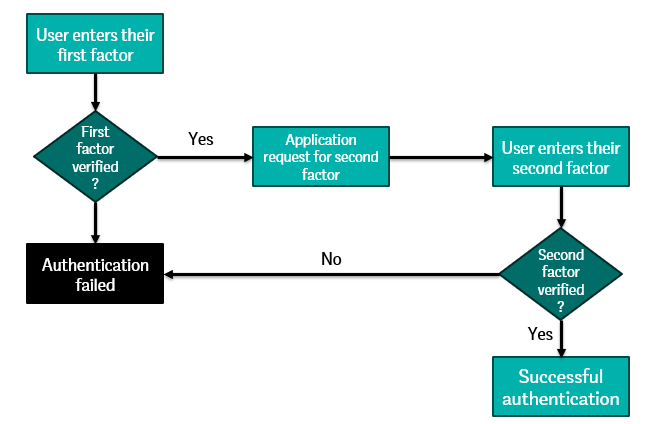
\includegraphics[width=0.8 \linewidth]{Images/K4/mfa-diagram.png}
	\caption{Multi-Factor Authentication Workflow}
	\label{fig:mfa_workflow}
\end{figure}

Commonly used as a complementary authentication factor to passwords, time-based one-time passwords, or TOTP, is an authentication standard where users receive a random constantly changing code, either through a mobile application or a hardware device, which confirms the user's identity, as long as the secret code and the current time between the user device and the authentication server are roughly the same \cite{gilman_zero_2017}. This authentication factor is specifically introduced, since it plays a crucial role in the MFA process of the practical implementation in Chapter 4.

\subsubsection{Micro-Segmentation}
Micro-segmentation is the process of dividing a network into smaller and isolated network segments, which are protected by their own security settings. With the view to restrict the lateral movement inside a network, micro-segmentation divides the network into zones based on separate policies. Access to a segment of the network is only granted predicated on the identity and predefined user behaviour.\\
This serves to minimize the attack surface for each segment of the network, however, more importantly, to contain eventual breaches in a single network segment. By dividing the network into several small segments, this also makes anomalies in the network much more visible.

\subsubsection{Identity and Access Management (IAM)}
The IAM component in the Zero Trust model controls which specific resources only authorized users can access in the network. It ensures the user's identity is verified correctly and utilizes role-based access control (RBAC) to ensure that the access a user has been granted is well within their role in the organization.\\
The benefits of such a process vary from centralizing the control over users' access to resources to enhancing the synergy between the other ZT model components by enforcing least privilege access and allowing straightforward monitoring of user behaviour.

\subsubsection{Least Privilege Access}
The principle of least privilege is defined by the provision of the minimum permissions to users required to finish a certain task. This granular access is adjusted based on a user's role within the organization and is usually enforced by the IAM system. Permissions within the network are dynamically adjusted, meaning that they are updated in real-time, according to user behaviour and their security status. This ensures that no standing user privileges can compromise sensitive information inside the network.\\
This aspect of the Zero Trust framework serves to minimize sensitive data exposure, in the case of user credentials being compromised. 

\subsubsection{Continuous Monitoring and Analytics}
While not considered a security feature in itself, the act of continuous monitoring is just as essential as the rest of the other components by providing real-time information for any unusual network activity, such as change of user location, revoked access, change in device health, etc. By utilizing this component, any potentially malicious anomaly in the network is quickly detected and managed accordingly -- usually by way of User and Entity Behavior Analytics (UEBA) and Security Information and Event Management (SIEM) tools.\\
This anomaly prevention process stands to improve the visibility of user activity within the network, allowing for the early detection of threats through logging and alerting for anomalous network activity.

\section{Fundamental Technologies and Concepts}
This section aims to provide additional information about a collection of concepts and technologies, which are not a part of any specific category, however are just as relevant for this thesis work as the aforementioned topics around smart homes and Zero Trust.

\subsection{Home Assistant}
Originally developed by Paulus Schoutsen in 2013, “Home Assistant” is a free and open-source platform for home automation \cite{home_assistant_wiki}. It serves as a central management hub for IoT devices and various services, where they are connected through one interface. Home Assistant supports all major smart home solutions, including but not limited to Amazon Alexa, IKEA TRÅDFRI, Zigbee Home Automation (ZHA), etc.\\
It consists of 3 main components -- Operating System, Supervisor, and Core, as depicted in Figure 2.3. The operating system is the base Linux environment, which runs both Core and Supervisor. On the other hand, Supervisor is responsible for managing the operating system, while Core interacts with users and the variety of IoT devices and services. \cite{home_assistant_arch}

\begin{figure}[H]
	\centering
	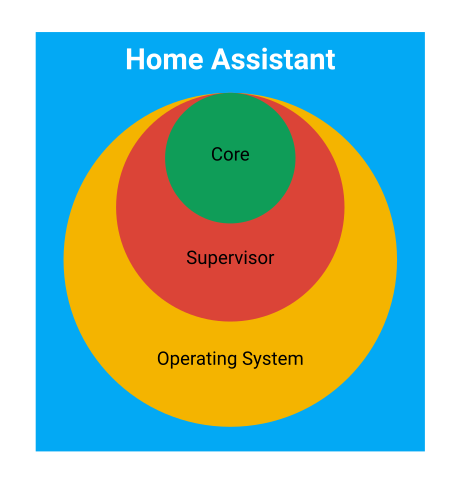
\includegraphics[width=0.5 \linewidth]{Images/ha_arch.png}
	\caption{Home Assistant architecture overview}
	\label{fig:Home_Ass_Arch}
    \cite{home_assistant_arch}
\end{figure}

\subsection{Raspberry Pi}
Originally intended for students to further develop their computer science skills, the “Raspberry Pi” (RPI) is a series of single-board computers (SBCs) with over 60 million devices sold \cite{raspberrypi_wiki}, \cite{raspberrypi_cnn}. The goal of this project is to provide a credit card-sized and mobile computing solution (Figure 2.4) with all relevant building blocks (Figure 2.5) and enough processing power to act as a standalone minicomputer workstation \cite{rpi_arch}.\\
\begin{figure}[H]
\centering
\begin{minipage}{.5\textwidth}
  \centering
  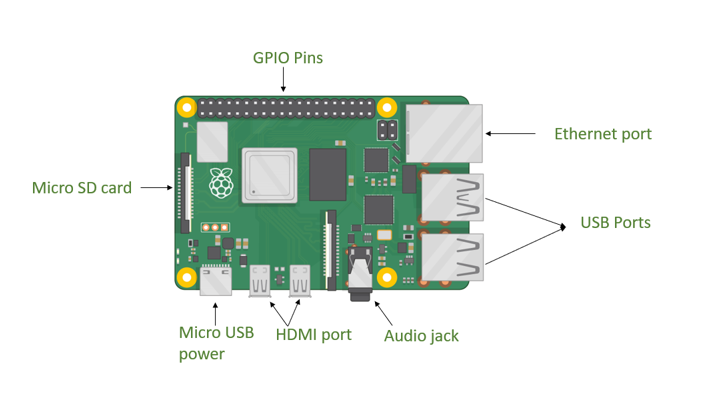
\includegraphics[width=0.7\linewidth]{Images/rasberrypi.png}
  \caption{Architecture of a Raspberry Pi}
  \label{fig:RPI_Arch}
  \cite{rpi_arch}
\end{minipage}%
\begin{minipage}{.5\textwidth}
  \centering
  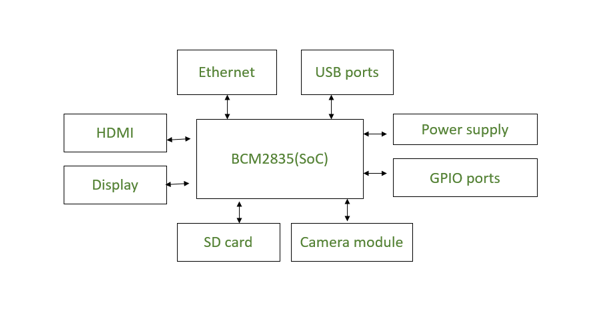
\includegraphics[width=0.8\linewidth]{Images/rasberrypi1.png}
  \caption{Main blocks of a Raspberry Pi}
  \label{fig:RPI_blocks}
  \cite{rpi_arch}
\end{minipage}
\end{figure}

Due to its large support community and ubiquitous usage in the field of smart homes, the RPI in the context of this thesis work is used to run the Home Assistant Operating System \cite{ha_os}. It is also responsible for the gateway-based communication with IoT devices and services, assuming the role of a central server for the on-premise smart home setup.

\subsection{Communication Protocols}
\subsubsection{Zigbee}
Based on the IEEE 802.15.4 standard for Low-Rate Wireless Personal Area Networks (LR-WPAN) \cite{ieee802154}, Zigbee is a wireless communication protocol, which has been specifically designed for small-scale personal area networks with low-power consumption devices in mind. In more detail, the Zigbee protocol is widely utilized in the integration of light bulbs, sockets, thermostats, and other smart devices, having established itself as a standard in home automation networks.\\
The devices within a Zigbee network are all dependent on a Zigbee gateway for their communication, which is connected to the Internet and serves as their controller node. However, they form a so-called mesh network, as shown in Figure 2.6 -- where the devices themselves act as routers, receiving and forwarding network requests -- thus ensuring the stability and reliability of the network. For a Zigbee setup to be regarded as complete, it must include 3 core components: the Zigbee gateway, which acts as an intermediary between the Internet and the smart devices, a coordinator device, usually either a smartphone or a tablet, to control and monitor the network remotely through a coordinator app (e.g. Home Assistant), and at least one end device as a component of the network itself \cite{zigbee_watt24}.

\begin{figure}[H]
	\centering
	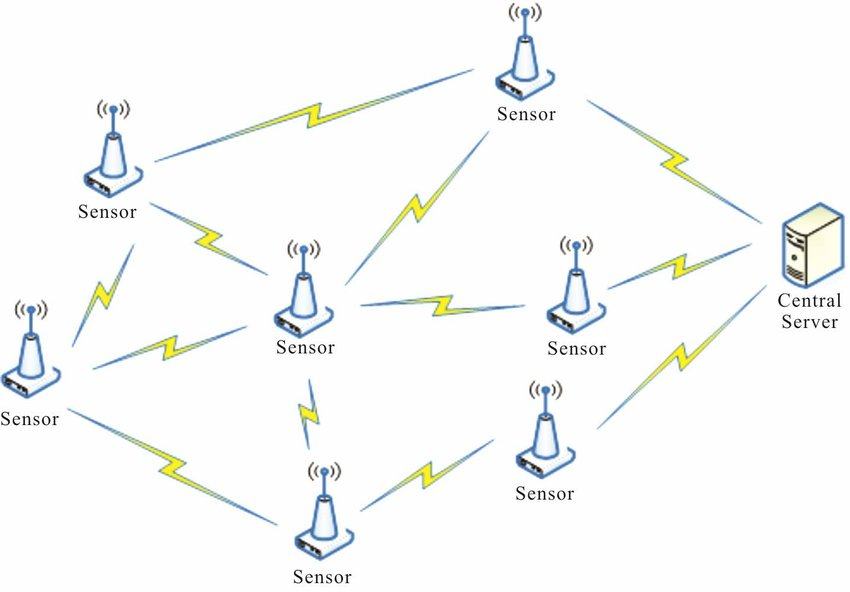
\includegraphics[width=0.5 \linewidth]{Images/ZigBee-mesh-network.jpg}
	\caption{Zigbee mesh network}
	\label{fig:Zigbee_Mesh}
    \cite{zigbee_mesh_network_article}
\end{figure}

\subsubsection{Bluetooth Low Energy}
Developed as an upgrade over Bluetooth 4.0 and above, Bluetooth Low Energy (BLE) has become the de facto Bluetooth technology for low-power devices \cite{bluetooth_le}, also being adopted as a communication protocol for IoT devices as a result.\\
In contrast to Zigbee, BLE does not require a separate gateway to establish the connection to smart devices, since the user device (usually a smartphone or an RPI) can already communicate per Bluetooth. This small difference makes the use of BLE devices, especially for its wide compatibility and straightforwardness, more convenient to set up and use than Zigbee. However, as the Zigbee protocol was designed with home automation in mind, BLE devices are best suited for infrequent communication between battery-powered devices, such as wireless headphones or smartwatches, which incorporate a wide variety of sensors \cite{bluetooth_v_zigbee}. Conversely, Zigbee devices most commonly consist of one or several sensors with a specific niche application, e.g. room environment metrics.

\subsubsection{MQTT}
The MQTT (Message Queuing Telemetry Transport) protocol is a Publish/Subscribe messaging protocol. Due to it being a lightweight protocol with a simple implementation, it is possible to run on devices without an operating system (OS), making it ideal for IoT applications. The central part of the MQTT network is the MQTT \textit{broker}, which acts as the server, receiving and distributing the messages between MQTT clients (either mobile devices or other backend systems) \cite{aigner_hacking_2018}.\\
The client communication is based on the concept of \textit{topics} -- as the data is organized in a tree-based topology, a topic is essentially the leaf node, which saves the data transmitted by the device. IoT devices then \textit{publish} their data over a corresponding topic for the broker to store, which in turn would forward it to all devices currently \textit{subscribed} to the given topic.\\
Figure 2.7 depicts an example of the MQTT Publish/Subscribe architecture, where a temperature sensor publishes its updated temperature data to the \textit{'temperature'} topic. The broker then publishes the changed value of the data for the other two clients, which are subscribed to that particular topic. 

\begin{figure}[H]
	\centering
	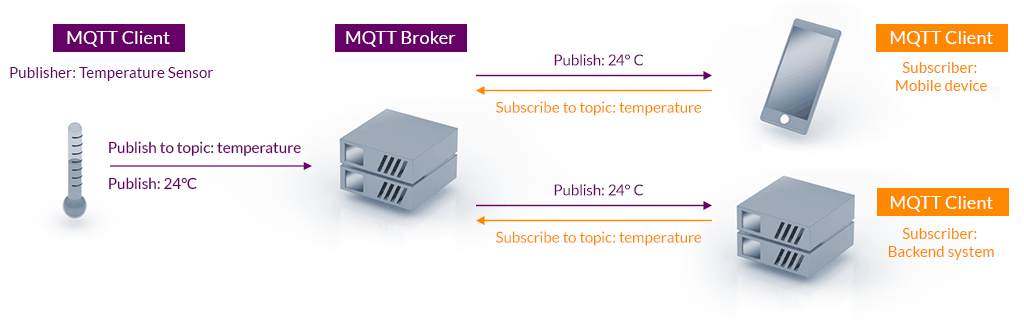
\includegraphics[width=0.9 \linewidth]{Images/mqtt-publish-subscribe.png}
	\caption{MQTT Publish/Subscribe Architecture}
	\label{fig:MQTT_Arch}
    \cite{mqtt_arch}
\end{figure}

\subsection{Infrastructure-as-a-Service}
Infrastructure-as-a-Service (IaaS) is a business model, which delivers hardware resources, such as processing power, storage and network resources, on virtual servers over the Internet. By employing the services of an IaaS provider, users benefit by not having to provide and manage physical IT infrastructure and instead work on the deployment and support of their own applications. This makes clients solely in charge of the software stack. \cite{aws_iaas}

\subsubsection{Elastic Compute Cloud}
Elastic Compute Cloud (EC2) is the IaaS solution of Amazon Web Services (AWS), setting the norm for public cloud computing solutions in 2006. EC2 offers virtual servers that allow users to host a Linux or Windows OS of their choice, with all compatible software accessible as well. According to the users' needs, EC2 offers a plethora of instance types \cite{aws_instances} through Amazon Machine Images (AMI), which serve as OS images for the virtual machines; the deployment of virtual machines (VMs) and virtual networks can then be finetuned and expanded upon with storage devices, load balancing, an autoscaling configuration, etc. \cite{stender2020cloud}

\subsection{Infrastructure-as-Code}
The Infrastructure-as-Code (IaC) paradigm contributes to the IaaS model by enabling the allocation and management of resources for in the cloud using template source files. This involves the automation of the infrastructure configuration with a view to minimize errors and establish a convention for the resources of virtual servers to be restored and reproduced identically. As the adoption of those principles is based on configuration scripts, practices from the field of software development, such as version control and syntax checking, have been integrated into the workflow of IaC tools. \cite{stender2020cloud}

\subsubsection{Terraform}
Terraform, developed by HashiCorp Inc., is an IaC tool that can be used to define both cloud and on-premise resources in human-readable configuration files for managing IT infrastructure throughout its whole development lifecycle \cite{tf_intro}.\\
Since this is a command-line interface (CLI) application, it can be directly embedded into the IaC workflow, enabling the flexibility of provisioned infrastructure with a few script lines. Terraform supports all major IaaS services of cloud providers, including Amazon Web Services, owing to its abundance of both official and community plugins to make compatibility one of its most appealing features. \cite{stender2020cloud}\\
Utilizing a declarative programming style, the Terraform framework is divided in 3 main stages: write, plan, and apply, as shown in Figure 2.8. Terraform scripts are written to describe the desired end state of the infrastructure in configuration files, with the code itself partially serving as documentation for the configuration settings. The writing stage defines the resources to be provisioned by the service provider, ranging from the low-level aspects, including, but not limited to the number of virtual CPUs, memory, and storage to the network architecture -- CIDR blocks, subnets, inbound/outbound traffic rules, etc. Subsequently, the planning stage provides a preview of the changes for the user.\\
The last stage of applying the changes provisions the infrastructure to the IaaS provider and updates the state file \cite{tf_state}, which is primarily used for storing the bindings between objects in a remote system and resource instances declared in the user's configuration. The purpose of this is to enable Terraform to know which resources are under its control, when to update and when to destroy them, streamlining the provisioning process \cite{tf_state_2}.

\begin{figure}[H]
	\centering
	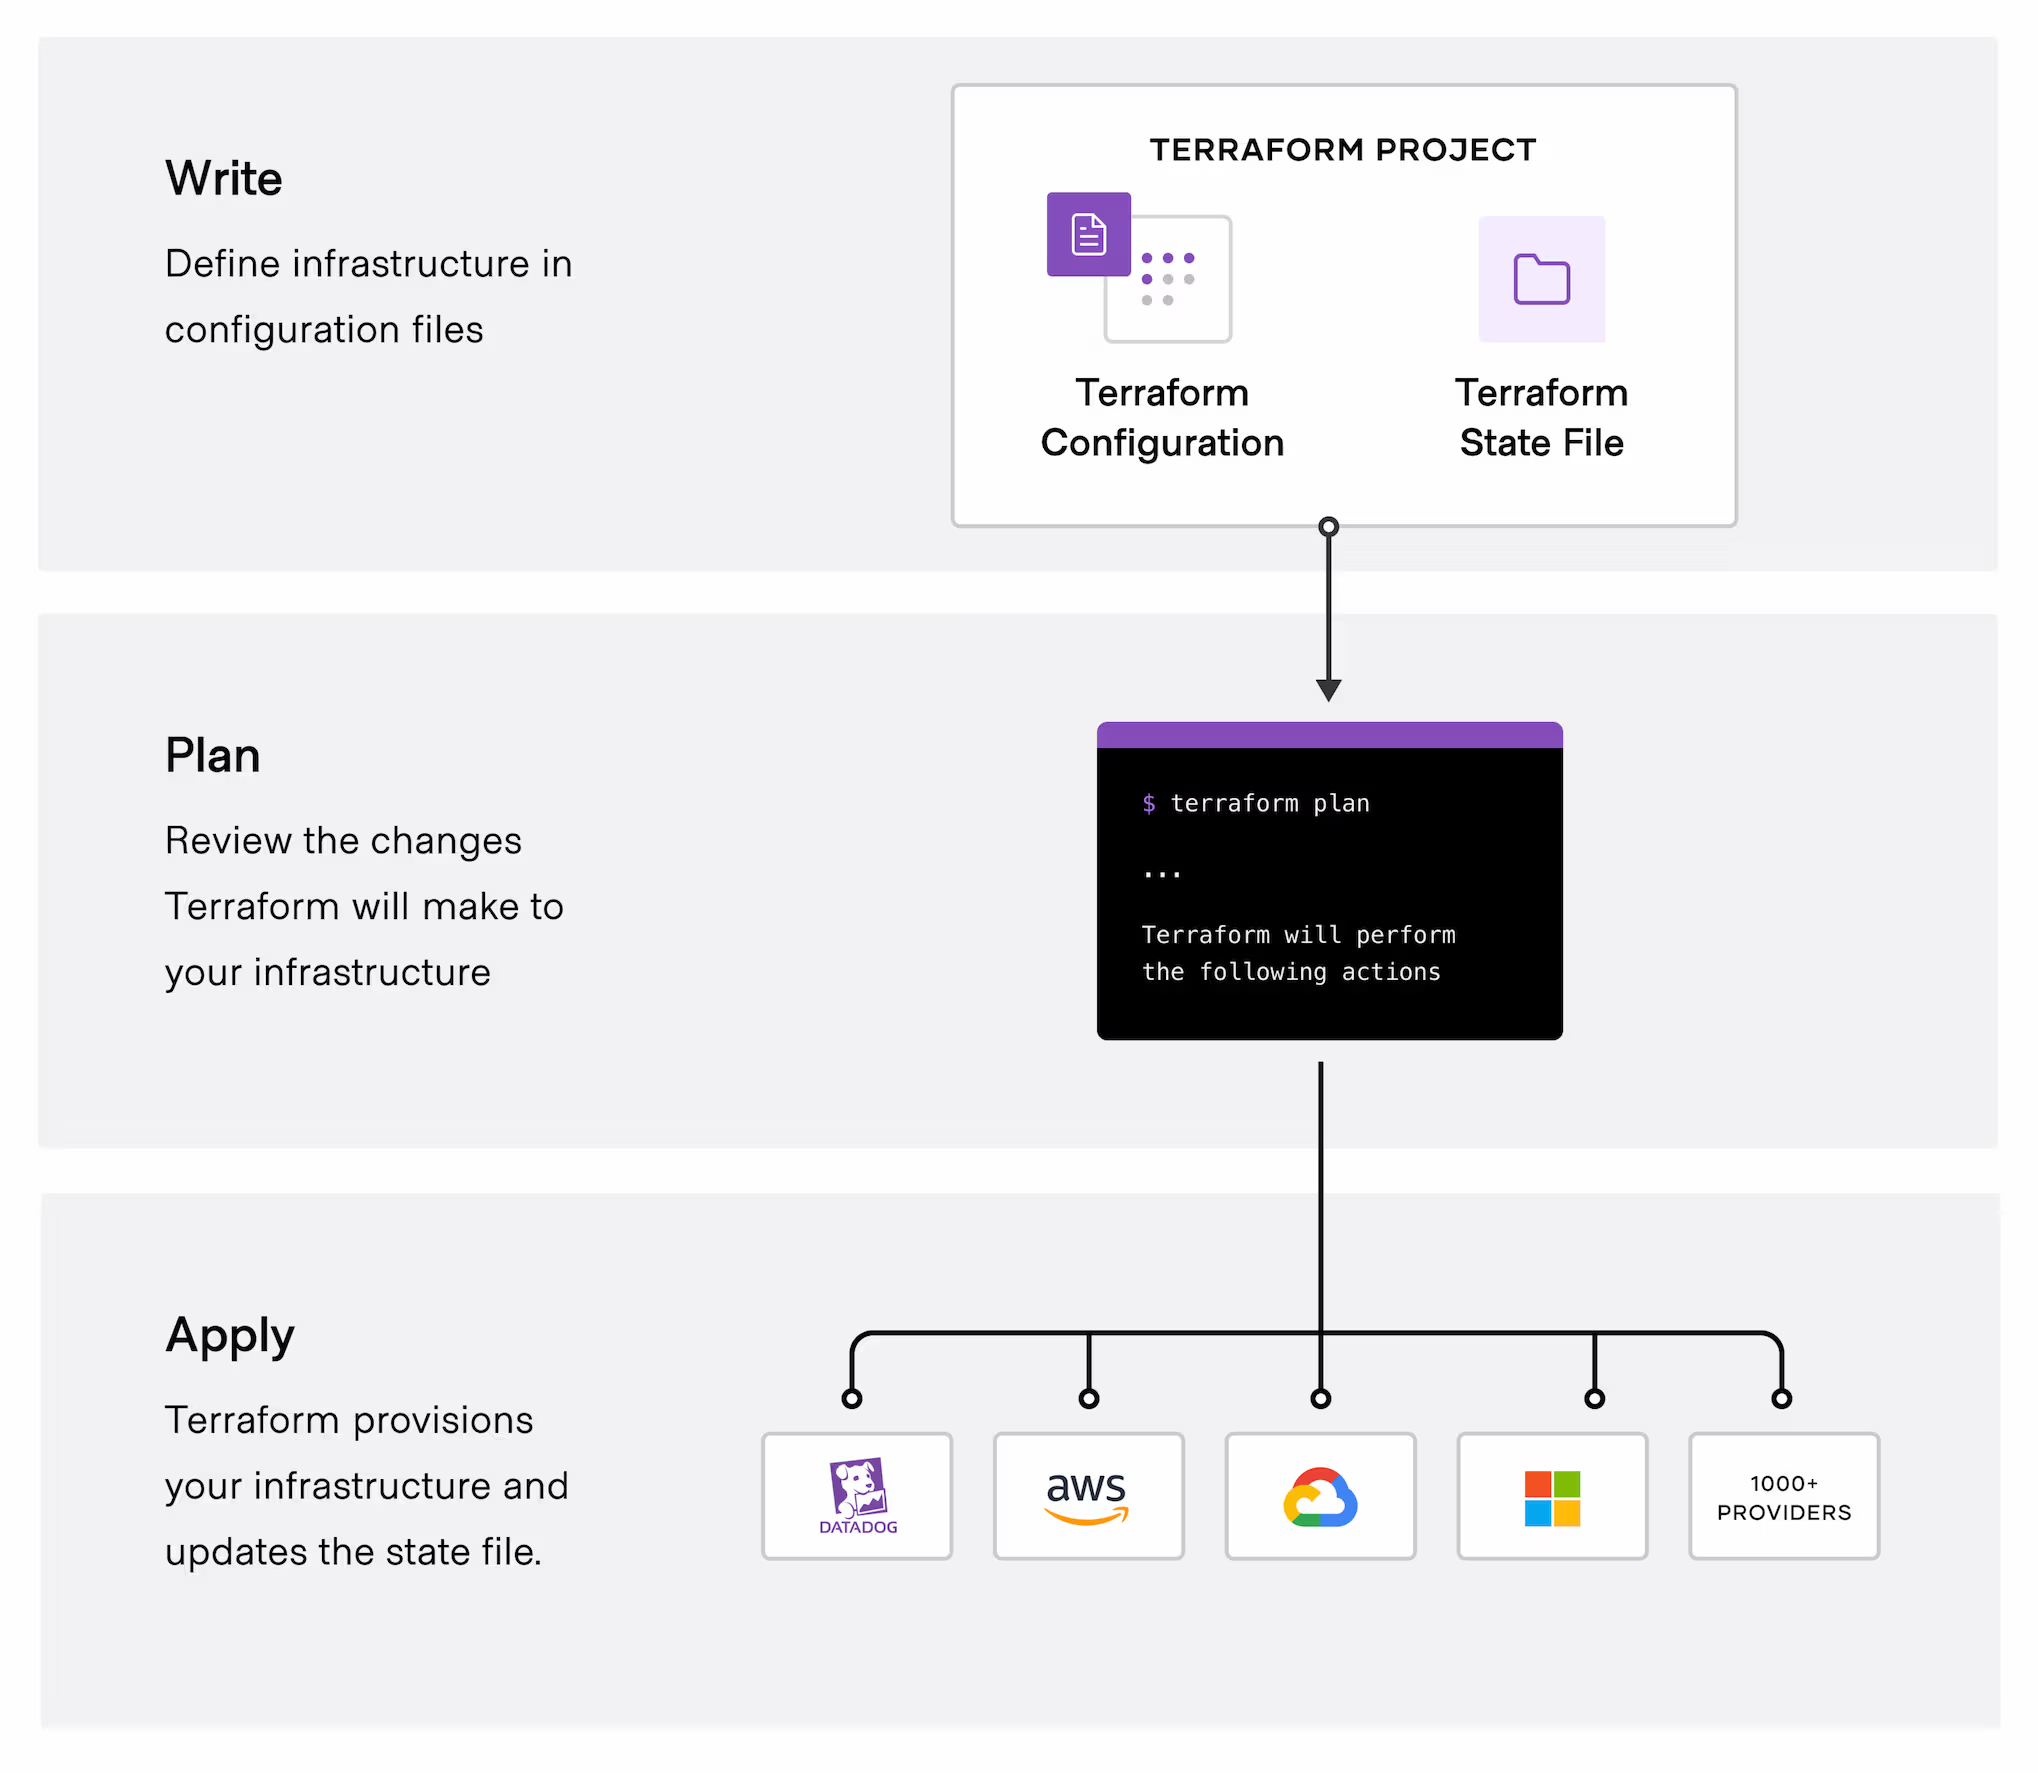
\includegraphics[width=0.8 \linewidth]{Images/tf_workflow.png}
	\caption{Terraform Workflow}
	\label{fig:Tf_workflow}
    \cite{tf_intro}
\end{figure}

\subsection{Containerization}
Containerization is the process of “packaging” a software application with all libraries and dependencies needed to run it into an executable called a \textit{container}. This method is widely adopted to universally deploy applications more swiftly and securely on any IT infrastructure as a single entity. \cite{ibm_container}\\
The entire container entity then runs encapsulated in a separate runtime environment with its own file system, isolated from the host system. A container is launched from a so-called \textit{container image}, which is the amalgamation of the software application with its runtime environment, the OS, all library and file dependencies in a lightweight base system. This means that a \textit{container} is simply an instance of an image, although the two terms are usually used interchangeably. The individual container images are usually distributed over a \textit{container registry}, e.g. Docker Hub, allowing them to be imported locally on the host. \cite{stender2020cloud}\\

\subsubsection{Docker Compose}
As part of the Docker platform, Docker Compose is the tool for defining and running applications, comprised of several containers. With the goal to simplify the control over these multi-container applications, all configuration is done in a single YAML configuration file, most commonly known as \textit{docker-compose.yml}, where the desired environment for the application has been specified. \cite{compose}\\
Docker Compose interacts with the applications in the Docker CLI, by using the \textit{docker compose} command and its subcommands, allowing users to effortlessly start, stop and configure their applications \cite{how_compose_works}.\\
Figure 2.9 outlines the overall workflow for Docker Compose. After the configuration file has been defined, Docker Compose will then build and run all the needed images based on it, and then create the environment for the application, including the container setup, any network settings required for the application's services and occasionally data volumes for persistent data storage provided that containers are restarted \cite{docker_compose_blog}.

\begin{figure}[H]
	\centering
	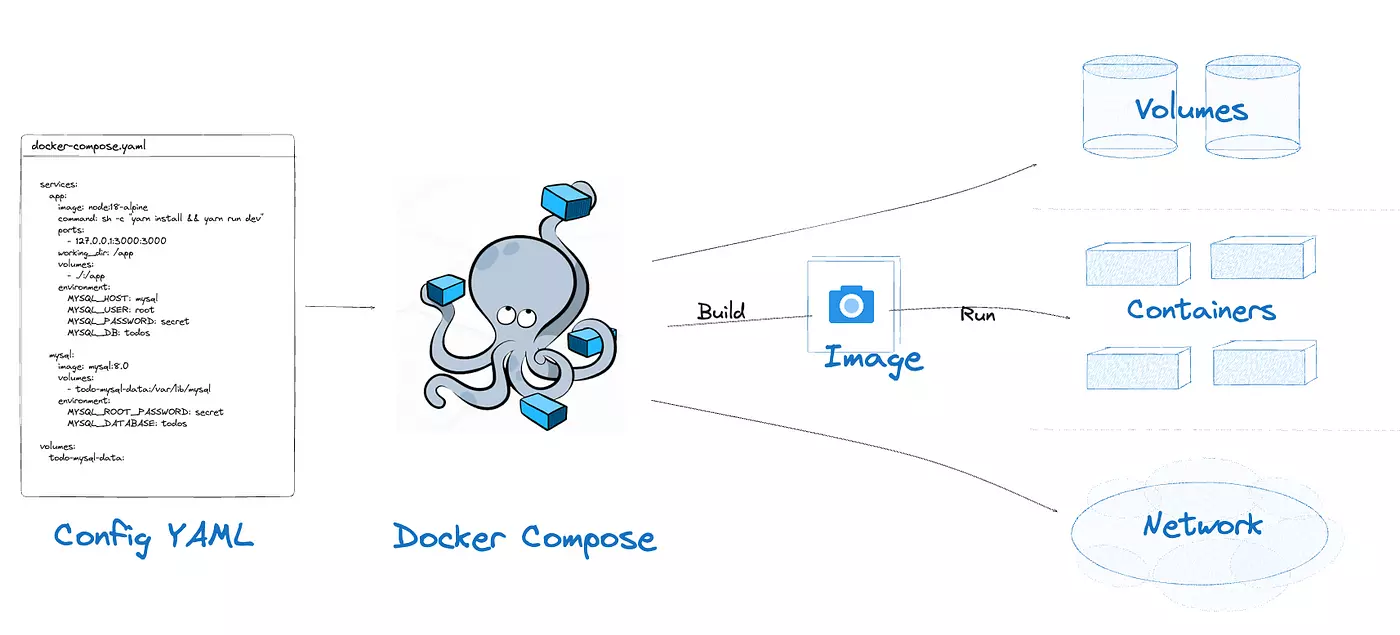
\includegraphics[width=0.8 \linewidth]{Images/docker-compose-flow.png}
	\caption{Docker Compose Workflow}
	\label{fig:dockerC_workflow}
    \cite{docker_compose_blog}
\end{figure}